%&tex

\documentclass{beamer}

\usepackage[english]{babel}
\usepackage[utf8]{inputenc}
\usepackage{mathtools}
\usepackage{amsthm}
\usepackage{amssymb}
\usepackage{thmtools,thm-restate}
\usepackage{amsfonts}
\usepackage{hyperref}
\usepackage[singlelinecheck=false]{caption}
\usepackage[backend=biber,url=true,doi=true,eprint=false,style=authoryear]{biblatex}
\usepackage{algorithm}
\usepackage[noend]{algpseudocode}
\usepackage{listings}
\usepackage{subcaption}

\usepackage{graphicx}
\usepackage{tikz}
\usetikzlibrary{positioning}
\usetikzlibrary{shapes.geometric}
\usetikzlibrary{fit}
\usetikzlibrary{calc}

\addbibresource{references.bib}
\usetheme{metropolis}

\DeclareMathOperator*{\argmin}{arg\,min}
\DeclareMathOperator*{\argmax}{arg\,max}
\DeclareMathOperator*{\Val}{\text{Val}}
\DeclareMathOperator*{\Ch}{\text{Ch}}
\DeclareMathOperator*{\Pa}{\text{Pa}}
\DeclareMathOperator*{\Sc}{\text{Sc}}
\newcommand{\ov}{\overline}
\newcommand{\tsup}{\textsuperscript}

\newcommand\defeq{\mathrel{\overset{\makebox[0pt]{\mbox{\normalfont\tiny\sffamily def}}}{=}}}

\newcommand{\algorithmautorefname}{Algorithm}
\algrenewcommand\algorithmicrequire{\textbf{Entrada}}
\algrenewcommand\algorithmicensure{\textbf{Saída}}
\algrenewcommand\algorithmicif{\textbf{se}}
\algrenewcommand\algorithmicthen{\textbf{então}}
\algrenewcommand\algorithmicelse{\textbf{senão}}
\algrenewcommand\algorithmicfor{\textbf{para todo}}
\algrenewcommand\algorithmicdo{\textbf{faça}}
\algnewcommand{\LineComment}[1]{\State\,\(\triangleright\) #1}

\newcommand{\Left}{\text{LEFT}}
\newcommand{\Right}{\text{RIGHT}}
\newcommand{\Up}{\text{UP}}

\newcommand{\set}[1]{\mathbf{#1}}
\newcommand{\pr}{\text{P}}
\newcommand{\eps}{\varepsilon}
\newcommand{\ddspn}[2]{\frac{\partial#1}{\partial#2}}
\newcommand{\iddspn}[2]{\partial#1/\partial#2}
\newcommand{\indep}{\perp}
\renewcommand{\implies}{\Rightarrow}

\newcommand{\bigo}{\mathcal{O}}

\setbeamertemplate{theorems}[ams style]

\setbeamersize{description width=1.0cm}

\lstset{frameround=fttt,
	numbers=left,
	breaklines=true,
	keywordstyle=\bfseries,
	basicstyle=\ttfamily,
}

\newcommand{\code}[1]{\lstinline[mathescape=true]{#1}}
\newcommand{\mcode}[1]{\lstinline[mathescape]!#1!}

\title{Mobile Robot Self-Driving Through Image Classification Using Discriminative Learning of
Sum-Product Networks}
\date{}
\author{Student: Renato Lui Geh\\Advisor: Prof. Denis Deratani Mauá}
\institute{Institute of Mathematics and Statistics --- University of São Paulo}

\begin{document}

\maketitle

\begin{frame}
  \frametitle{In an Ideal world...}

  \begin{align*}
    \overbrace{\overbrace{\overbrace{\textbf{Mobile Robot}}^{1}\text{ }
    \overbrace{\textbf{Self-Driving}}^{2}}^{3}\textbf{ Through }
    \overbrace{\textbf{Image Classification}}^{4}}^{5}\\\textbf{ Using }
    \underbrace{\underbrace{\textbf{Discriminative Learning}}_{6}\textbf{ of }
    \underbrace{\textbf{Sum-Product Networks}}_{7}}_{8}
\end{align*}
\end{frame}

\begin{frame}
  \frametitle{...but life is short}

  \begin{align*}
    \overbrace{\textbf{Mobile Robot Self-Driving Through Image Classification}}^{\text{Section 2}}\\
    \underbracket{\textbf{Using Discriminative Learning of }\underbrace{\textbf{Sum-Product
    Networks}}_{\text{Section 1}}}_{\text{Section 3: }(1+2)}
  \end{align*}
\end{frame}

\section{Sum-Product Networks}

\begin{frame}
  \frametitle{Definition}
  \begin{definition}[\cite{gens-domingos}]~\\
    A sum-product network (SPN) is a DAG where each node can be defined recursively as follows.
    \begin{enumerate}
      \item A tractable univariate probability distribution is an SPN\@.
      \item A product of SPNs with disjoint scopes is an SPN\@.
      \item A weighted sum of SPNs with the same scope is an SPN, provided all weights are positive.
      \item Nothing else is an SPN\@.
    \end{enumerate}
  \end{definition}
\end{frame}

\begin{frame}
  \frametitle{Sum-product network}

  The value $S(X)$ of an SPN is equal to $\phi(X)$, an unnormalized probability function, if it
  obeys certain properties. If all weights sum to one, $S(X)=P_{\phi}(X)$ (\cite{poon-domingos}).

  \begin{figure}
    \centering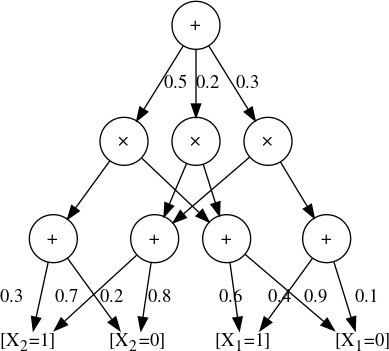
\includegraphics[height=0.6\textheight]{imgs/sample_spn.png}
  \end{figure}
\end{frame}

\begin{frame}
  \frametitle{Probability of evidence}

  Single forward pass computes $S(X=\{X_1=0\})=0.31$. Linear on the number of edges

  \begin{figure}
    \centering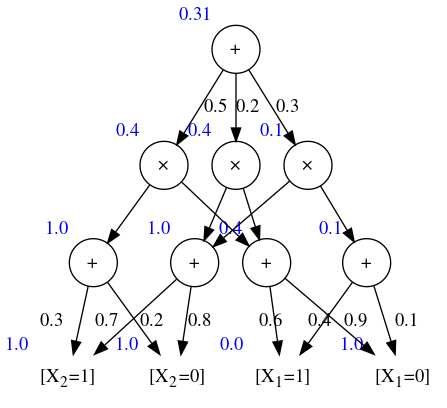
\includegraphics[height=0.6\textheight]{imgs/sample_spn_prob.png}
  \end{figure}
\end{frame}

\begin{frame}
  \frametitle{Maximum a posteriori probability}

  Replace sums with max nodes. Forward pass followed by backward pass computes most probable
  explanation, i.e. find $\argmax_{x\in X} P(X, E)$.

  \begin{figure}
    \centering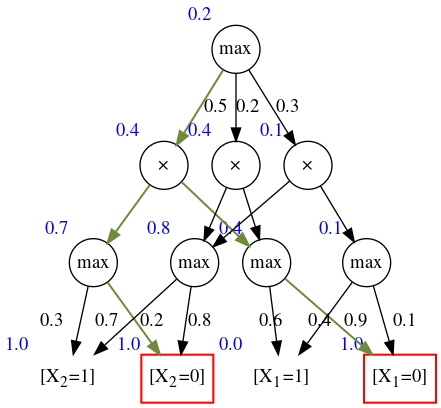
\includegraphics[height=0.6\textheight]{imgs/sample_mpn_prob.png}
  \end{figure}
\end{frame}

\begin{frame}
  \frametitle{Learning}

  \textbf{Structure}
  \begin{itemize}
    \item PD-Dense architecture (\cite{poon-domingos})
    \item \textbf{Clustering on Variables} (\cite{clustering})
    \item \textbf{Gens-Domingos LearnSPN} (\cite{gens-domingos})
    \item Using deep learning techniques (\cite{deep-learn-spn})
    \item many others...
  \end{itemize}

  \textbf{Weights}
  \begin{itemize}
    \item \textbf{Generative and discriminative gradient descent}
    \item Generative Expectation-Maximization
    \item Extended Baum-Welch (\cite{baum-welch})
    \item many others...
  \end{itemize}
\end{frame}

\section{Self-Driving}

\begin{frame}
  \frametitle{Self-driving as image classification}

  Let $X=\{X_0,X_1,\ldots,X_{n-1}\}$ be an \textbf{image}. Every $X_i=x_i$ refers to the $i$-th
  pixel with a grayscale intensity of $x_i$.

  Let $Y=\{\Up,\Left,\Right\}$ be the \textbf{classification variable}.

  \begin{figure}
    \begin{subfigure}{0.3\linewidth}
      \centering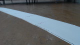
\includegraphics{imgs/sample_left.png}
      \captionsetup{justification=centering}
      \caption*{LEFT}
    \end{subfigure}
    \begin{subfigure}{0.3\linewidth}
      \centering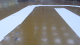
\includegraphics{imgs/sample_up.png}
      \captionsetup{justification=centering}
      \caption*{UP}
    \end{subfigure}
    \begin{subfigure}{0.3\linewidth}
      \centering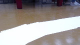
\includegraphics{imgs/sample_right.png}
      \captionsetup{justification=centering}
      \caption*{RIGHT}
    \end{subfigure}
  \end{figure}

  The entire scope of variables is $X\cup Y$.

  \vfill\centering\textbf{Objective:} $\argmax_{y\in Y} P(Y=y|X)$
\end{frame}

\begin{frame}
  \frametitle{Dataset}

  Dataset used: \cite{self-driving}

  \begin{figure}
    \centering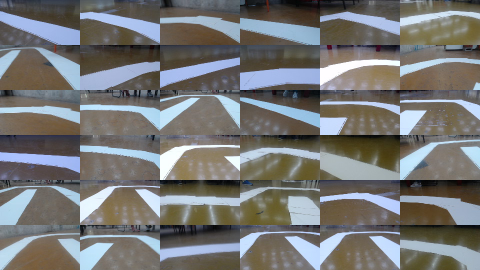
\includegraphics[height=0.5\textheight]{imgs/montage_raw.png}
  \end{figure}

  Lane tracking dataset with $80\times 45$ RGB images. Each labeled with either UP, LEFT or RIGHT.
\end{frame}

\begin{frame}
  \frametitle{Pre-processing}

  \textbf{Pipeline:}

  \centering{original RGB image $\to$ grayscale $\to$ some $T$ transformation.}

  \flushleft Three transformations tested:
  \begin{enumerate}
    \item Otsu binarization (\cite{otsu})
    \item Quantization (resolution downscaling)
    \item Histogram equalization
  \end{enumerate}

  \begin{figure}
    \begin{subfigure}{0.3\linewidth}
      \centering
\includegraphics{imgs/binary_up.png}
      \captionsetup{justification=centering}
      \caption*{1}
    \end{subfigure}
    \begin{subfigure}{0.3\linewidth}
      \centering
\includegraphics{imgs/trans_up.png}
      \captionsetup{justification=centering}
      \caption*{2}
    \end{subfigure}
    \begin{subfigure}{0.3\linewidth}
      \centering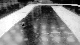
\includegraphics{imgs/eq_up.png}
      \captionsetup{justification=centering}
      \caption*{3}
    \end{subfigure}
  \end{figure}
\end{frame}

\begin{frame}
  \frametitle{Berry}

  \textbf{Raspberry Pi 3 Model B --- Berry}
  \begin{description}
    \item[CPU:] Quad Core 1.2GHz Broadcom BCM2837 64bit ARMv7
    \item[Memory:] 1GB RAM
    \item[Storage:] 16GB SSD
  \end{description}

  \begin{figure}
    \centering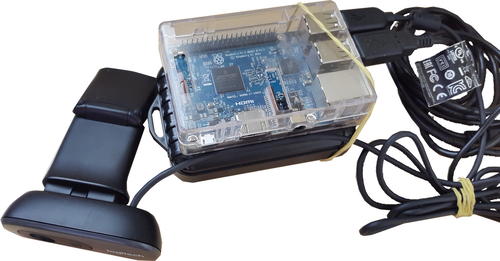
\includegraphics[height=0.4\textheight]{imgs/berry.png}
  \end{figure}
\end{frame}

\begin{frame}
  \frametitle{Brick}

  \textbf{Lego Mindstorms NXT v2 --- Brick}
  \begin{description}
    \item[CPU:] Atmel AT91SAM7S256 48MHz 32bit ARMv4
    \item[Memory:] 64KB RAM
    \item[Storage:] 256KB Flash
  \end{description}

  \begin{figure}
    \centering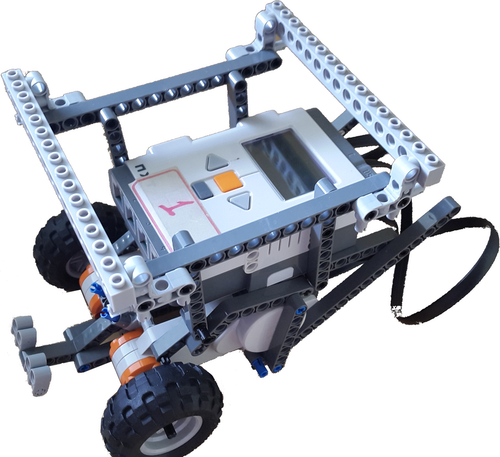
\includegraphics[height=0.4\textheight]{imgs/brick.png}
  \end{figure}
\end{frame}

\begin{frame}
  \frametitle{Robot}

  \textbf{Berry} handles inference, passing predicted label to \textbf{Brick}.

  \textbf{Brick} handles motors according to label received from \textbf{Berry}.

  \begin{figure}
    \centering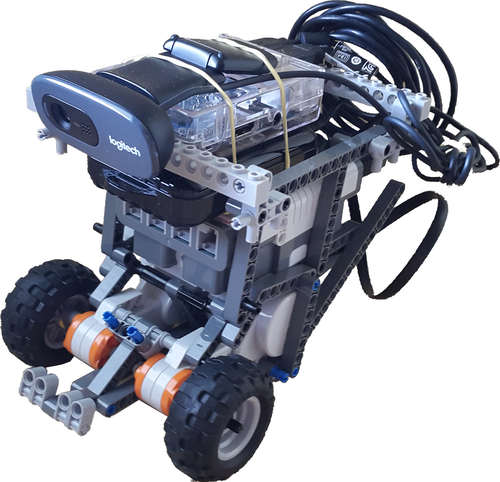
\includegraphics[height=0.5\textheight]{imgs/robot.png}
  \end{figure}

  \centering Message passing through USB cable.
\end{frame}

\section{Driving with SPNs}

\begin{frame}
  \frametitle{Modelling}

  Every pixel $X_i$ is a variable in the distribution represented by the SPN, i.e. no additional
  feature extraction, end-to-end.

  Two architectures:
  \begin{description}
    \item[GD:] LearnSPN (\cite{gens-domingos})
    \item[DV:] Clustering on Variables (\cite{clustering})
  \end{description}
  Three weight setups:
  \begin{description}
    \item[g:] Generative gradient descent (\cite{poon-domingos})
    \item[d:] Discriminative gradient descent (\cite{discriminative})
    \item[s:] Proportional weights for GD, random weights for DV
  \end{description}
\end{frame}

\begin{frame}
  \frametitle{Accuracy}
  \footnotesize
  \begin{table}[h]
    \centering
    \begin{tabular}{l|c|c|c|c|c|c}
      \hline
      \multicolumn{1}{c}{\bfseries Accuracy (\%)} & \multicolumn{1}{c}{\bfseries DV+g} &
      \multicolumn{1}{c}{\bfseries DV+d} & \multicolumn{1}{c}{\bfseries DV+s} &
      \multicolumn{1}{c}{\bfseries GD+g} & \multicolumn{1}{c}{\bfseries GD+d} &
      \multicolumn{1}{c}{\bfseries GD+s}\\
      \hline
      $B$         & 78.8 & 78.8 & 78.8 & 82.8 & 83.8 & 85.0\\
      $Q_2$       & 78.6 & 78.0 & 78.0 & 78.6 & 80.4 & 79.4\\
      $Q_2+E$     & 76.6 & 76.6 & 76.8 & 79.6 & 82.8 & 81.8\\
      $Q_3$       & 77.4 & 77.4 & 77.4 & 77.6 & 80.2 & 79.8\\
      $Q_3+E$     & 70.4 & 76.6 & 76.6 & 79.2 & 81.2 & 77.4\\
      $Q_4$       & 78.2 & 78.4 & 78.2 & 76.0 & 78.2 & 76.4\\
      $Q_4+E$     & 76.6 & 76.6 & 76.8 & 76.0 & 74.6 & 80.6\\
      $Q_5$       & 77.8 & 78.4 & 78.4 & 77.6 & 74.0 & 73.8\\
      $Q_5+E$     & 76.6 & 76.6 & 76.6 & 72.0 & 72.8 & 72.0\\
      $Q_6$       & 77.4 & 78.4 & 78.4 & 75.2 & 74.4 & 72.0\\
      $Q_6+E$     & 76.0 & 76.4 & 76.4 & 73.0 & 75.0 & 73.6\\
      $Q_7$       & 78.2 & 78.4 & 78.4 & 62.8 & 72.2 & 71.4\\
      $Q_7+E$     & 76.2 & 76.4 & 76.4 & 70.6 & 71.4 & 71.6\\
      $\emptyset$ & 78.0 & 78.4 & 78.4 & 62.4 & 62.4 & 62.4\\
      $E$         & 76.4 & 76.4 & 76.4 & 60.4 & 60.0 & 61.2\\
    \end{tabular}
  \end{table}
\end{frame}

\begin{frame}
  \frametitle{Inference time}
  \footnotesize
  \begin{table}[h]
    \centering
    \begin{tabular}{l|c|c|c|c|c|c}
      \hline
      \multicolumn{1}{c}{\bfseries Inference (secs)} & \multicolumn{1}{c}{\bfseries DV+g} &
      \multicolumn{1}{c}{\bfseries DV+d} & \multicolumn{1}{c}{\bfseries DV+s} &
      \multicolumn{1}{c}{\bfseries GD+g} & \multicolumn{1}{c}{\bfseries GD+d} &
      \multicolumn{1}{c}{\bfseries GD+s}\\
      \hline
      $B$         & 0.23 & 0.25 & 0.25 & 0.38 & 0.37 & 0.31 \\
      $Q_2$       & 0.22 & 0.24 & 0.23 & 0.28 & 0.34 & 0.16 \\
      $Q_2+E$     & 0.22 & 0.23 & 0.23 & 0.38 & 0.30 & 0.27 \\
      $Q_3$       & 0.22 & 0.23 & 0.22 & 0.22 & 0.32 & 0.17 \\
      $Q_3+E$     & 0.22 & 0.23 & 0.22 & 0.34 & 0.32 & 0.31 \\
      $Q_4$       & 0.22 & 0.22 & 0.23 & 0.16 & 0.17 & 0.13 \\
      $Q_4+E$     & 0.23 & 0.27 & 0.29 & 0.13 & 0.14 & 0.13 \\
      $Q_5$       & 0.22 & 0.26 & 0.28 & 0.07 & 0.05 & 0.02 \\
      $Q_5+E$     & 0.22 & 0.29 & 0.25 & 0.05 & 0.05 & 0.02 \\
      $Q_6$       & 0.23 & 0.24 & 0.23 & 0.04 & 0.05 & 0.01 \\
      $Q_6+E$     & 0.22 & 0.24 & 0.28 & 0.03 & 0.04 & 0.02 \\
      $Q_7$       & 0.23 & 0.23 & 0.26 & 0.03 & 0.01 & 0.01 \\
      $Q_7+E$     & 0.22 & 0.26 & 0.24 & 0.01 & 0.01 & 0.01 \\
      $\emptyset$ & 0.22 & 0.26 & 0.23 & 0.02 & 0.01 & 0.01 \\
      $E$         & 0.23 & 0.23 & 0.22 & 0.01 & 0.01 & 0.02 \\
    \end{tabular}
  \end{table}
\end{frame}

\begin{frame}
  \frametitle{``Real world'' scenario}

  \footnotesize\centering\textbf{\href{https://}{Mobile Robot Self-Driving Through Image Classification Using
  Discriminative Learning of Sum-Product Networks --- YouTube}}
\end{frame}

\begin{frame}[standout]
  \textbf{Thank you.\\~\\Questions?}
\end{frame}

\begin{frame}[t,allowframebreaks]
  \frametitle{References}
  \printbibliography[heading=none]
\end{frame}

\end{document}
